%! TEX root = ../thesis.tex

\chapter{The Pierre Auger Observatory}
\label{chap:auger-observatory}

Located on the argentinian high-plains of Pampa Amarilla, the Pierre Auger observatory is a hybrid detector designed to detect and study cosmic 
rays of the highest energies. With an effective area of \SI{3000}{\kilo\meter\squared} it is by far the largest experiment of its kind 
\cite{DesignReport}.

This chapter offers a brief look into the measurement principle and setup of the observatory. The  surface detector (SD) is described in 
\autoref{sec:surface-detector} and critical in understanding the analysis presented in \autoref{chap:station-triggers}. For a more complete 
overview on the experiment, information regarding the fluoresence detector can be found in \autoref{sec:fluoresence-detector}. Notes on the event
reconstruction are found in \autoref{sec:event-reconstruction}. If not explicitly stated otherwise, information is adpoted from the Pierre Auger 
observatory design report \cite{DesignReport}.

\section{Fluoresence Detector (FD)}
\label{sec:fluoresence-detector}

\begin{figure}
	\centering
	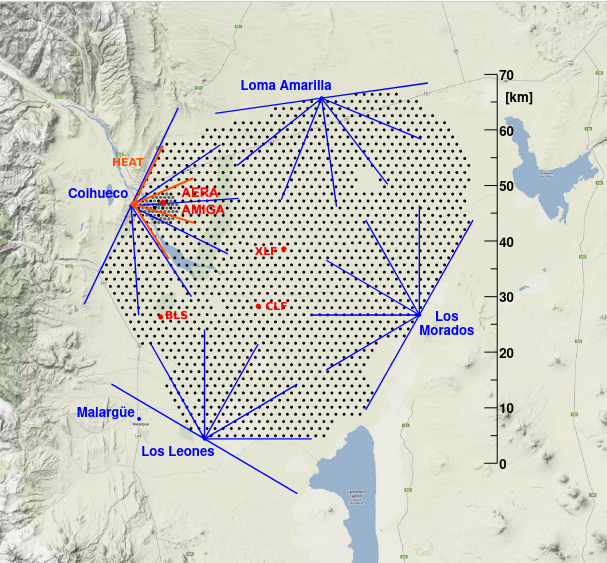
\includegraphics[width=0.9\textwidth]{plots/auger_array.png}
	\caption{Overview of the Pierre Auger observatory. The four different FD sites (respective FOV shown with blue lines) sit at the edge of
	the detector area and monitor the night sky above the SD array consisting of 1660 water tanks (black dots).}
	\label{fig:auger-array}
\end{figure}

The fluoresence detector are a total of 27 fluoresence telescopes at 4 different sites (compare \autoref{fig:auger-array}). Each telescope
monitors a \SI{30}{\degree} x \SI{30}{\degree} window of the night sky. This results in an effective FOV of roughly \SI{180}{\degree} x 
\SI{30}{\degree} per FD station, with an exception of Coihueco, where three additional telescopes (\textbf{H}igh \textbf{E}levation \textbf{A}uger
\textbf{T}elescope) are installed to monitor higher zenith angles ($\SI{30}{\degree}\leq\theta\leq\SI{60}{\degree}$) in order to increase
sensitivity for showers of lower energies (compare \autoref{chap:physical-background}).

The telescopes consists of a \SI{3.6}{\meter} by \SI{3.6}{\meter}, curved mirror, which reflect light onto 440 photomultipliers that make up the 
individual pixels of the photo sensor. In order to decrease 

\section{Surface Detector (SD)}
\label{sec:surface-detector}


